\chapter{مفاهیم پایه}
در این فصل به معرفی مفاهیم پایه موردنیاز برای درک قسمت‌های مختلف پروژه و جزییات پیاده‌سازی آن پرداخته می‌شود.

\newcommand{\dd}[1]{\mathrm{d}#1}

% Quantum Computation

\section{محاسبات کوانتومی}

\subsection{سیستم‌های تک‌کیوبیتی}

طبق قوانین فیزیک کوانتومی، حالت یک سیستم می‌تواند به صورت ترکیب خطی‌ای از چند حالت پایه باشد، که این حالت‌های پایه، حالت‌هایی هستند که در قوانین فیزیک کلاسیک نیز حالات صحیحی برای توصیف سیستم هستند.
در محاسبات کوانتومی از بردارهای عمودی برای نشان‌دادن وضعیت یک سیستم استفاده می‌شود و وضعیت سیستم‌های چندکیوبیتی را نیز می‌توان از روی بردارهای یک سیستم تک‌کیوبیتی نیز ساخت.
\\
به طور معمول، در محاسبات کوانتومی، با سیستم‌هایی با تنها دو حالت پایه سر و کار داریم، به همین علت، بردارهای فضای حالات سیستم‌های تک‌کیوبیتی ۲ بعدی هستند. لذا دو بردار مستقل یکه به عنوان بردارهای پایه‌ی این فضا تعیین داده می‌شوند که رابطه‌ی ۱-به-۱ ای با حالات پایه‌ی بیت‌های کلاسیک دارند.
این حالات پایه به صورت زیر تعیین می‌شوند:
\begin{equation}
    |0\rangle = \begin{bmatrix} 1 \\ 0 \end{bmatrix} 
    \mspace{18mu}
    |1\rangle = \begin{bmatrix} 0 \\ 1 \end{bmatrix}
\end{equation} 
\myequations{بردارهای پایه تک‌کیوبیتی}

نشان دادن بردارهای حالت به صورت 
\lr{$|0\rangle$} و \lr{$|1\rangle$}
به نمادگذاری \lr{bra-ket} دیراک
\fnote{Dirac's bra-ket notation}
معروف است و به ازای هر
\lr{ket}
به صورت زیر:
\begin{equation}
    |\psi\rangle = \alpha |0\rangle + \beta |1\rangle
    = \begin{bmatrix}
    \alpha \\[3pt]
    \beta
    \end{bmatrix}
\end{equation}
یک \lr{bra}
به این صورت تعریف می‌شود:
\begin{equation}
    \langle \psi| = \alpha^* \langle0| + \beta^* \langle1| = \begin{bmatrix} \alpha^* & \beta^* \end{bmatrix} 
\end{equation}

که در این‌جا نماد \lr{$\alpha^*$}
به معنای مزدوج مخلط 
\fnote{Complex conjugate}
عدد \lr{$\alpha$}
است.
\newpage

حالت‌های سیستم در فیزیک کوانتومی در اکثر اوقات به صورت بردارهای مختلط بهنجار
\fnote{Normalizable}
نشان داده می‌شوند.
\begin{equation}
    |\psi\rangle = \alpha |0\rangle + \beta |1\rangle = \begin{bmatrix} \alpha \\ \beta \end{bmatrix} 
    ; \mspace{18mu}
    \alpha, \beta \in \mathbb{C}
\end{equation}
% \newpage
\myequations{فرم کلی بردار وضعیت سیستم تک کیوبیتی}
که به امر ایجاد یک بردار وضعیت از ترکیب خطی دو بردار وضعیت دیگر، اصل برهم‌نهی کوانتومی
\fnote{Quantum Superposition}
گفته می‌شود.

بهنجار بودن به معنای صدق شرایط زیر است:
\begin{equation}
    \alpha\alpha^* + \beta\beta^* = |\alpha|^2 + |\beta|^2 = 1
\end{equation}
\myequations{شرط بهنجار بودن}
% \newpage
\begin{figure}
	\centering
	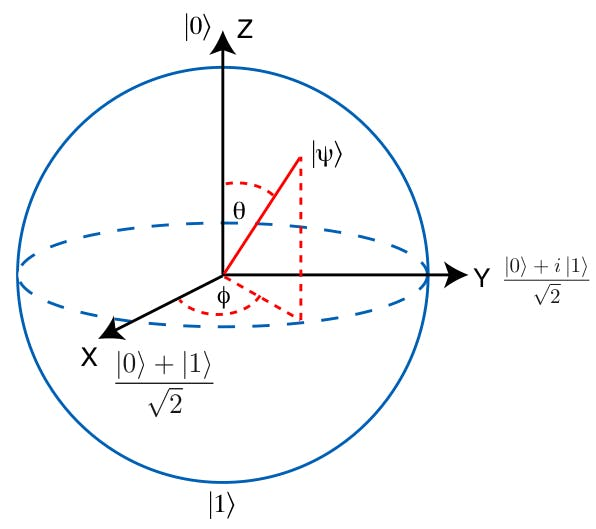
\includegraphics[scale=0.4]{figures/bloch.jpg}
	\caption{کره‌ی بلاخ}
	\label{fig:bloch}
\end{figure}
به علت شرط بهنجاری، می‌توان حالت کلی یک سیستم تک‌کیوبیتی را به صورت زیر نیز نوشت:
\begin{equation}
|\psi\rangle = \begin{bmatrix} e^{i\phi_1}\cos{\tfrac{\theta}{2}} \\[6pt] e^{i\phi_2}\sin{\tfrac{\theta}{2}} \end{bmatrix} 
\mspace{18mu}
\theta, \phi_1, \phi_2 \in {\rm I\!R}
\end{equation}
\myequations{حالت معادل فرم کلی بردار تک‌کیوبیتی}

که آن را می‌توان به صورت زیر نیز نوشت:
\begin{equation}
|\psi\rangle = e^{i\phi_1} \begin{bmatrix} \cos{\tfrac{\theta}{2}} \\[6pt] e^{i\phi_2-\phi_1}\sin{\tfrac{\theta}{2}} \end{bmatrix} = e^{i\phi_1} \begin{bmatrix} \cos{\tfrac{\theta}{2}} \\[6pt] e^{i\phi}\sin{\tfrac{\theta}{2}} \end{bmatrix}
\Rightarrow |\psi\rangle = \begin{bmatrix} \cos{\tfrac{\theta}{2}} \\[6pt] e^{i\phi}\sin{\tfrac{\theta}{2}} \end{bmatrix}
\end{equation}
\myequations{مهم نبودن فاز کلی سیستم}
در این معادله،
\lr{$\phi_1$}
 فاز کلی سیستم نامیده می‌شود که طبق قوانین فیزیک کوانتومی، در رفتار سیستم فاقد اهمیت است و به همین علت در مرحله‌ی آخر از آن صرف نظر شده‌است. \\
در نهایت، حالت کلی یک کیوبیت را می‌توان با استفاده از ابزاری به نام کره‌ی بلاخ (شکل
\ref{fig:bloch})
نمایش داد.

\subsection{سیستم‌های چندکیوبیتی}
اگر دو سیستم تک‌کیوبیتی جداگانه داشته باشیم، می‌توانیم آن‌ها را به صورت مجزا به صورت زیر تعریف می‌کنیم:
\begin{equation}
|a\rangle = \begin{bmatrix} a_0 \\ a_1 \end{bmatrix}, \quad |b\rangle = \begin{bmatrix} b_0 \\ b_1 \end{bmatrix}
\end{equation}
\myequations{دو کیوبیت مجزا}
در عین حال، می‌توانیم بردار وضعیت آن‌ها را به صورت هم‌زمان با استفاده از عملگری به نام ضرب تانسوری
\fnote{Tensor product}
تعریف کنیم که به صورت زیر عمل می‌کند:
\begin{equation}
|b\rangle \otimes |a\rangle = \begin{bmatrix} b_0 \times \begin{bmatrix} a_0 \\ a_1 \end{bmatrix} \\[12pt] b_1 \times \begin{bmatrix} a_0 \\ a_1 \end{bmatrix} \end{bmatrix} = \begin{bmatrix} b_0 a_0 \\[2pt] b_0 a_1 \\[2pt] b_1 a_0 \\[2pt] b_1 a_1 \end{bmatrix} = |ba\rangle
\end{equation}
\myequations{ضرب تانسوری}

\subsection{درهم‌تنیدگی}

درهم‌تنیدگی کوانتومی\fnote{Quantum Entanglement}
، یکی از اصول فیزیک کوانتومی است و به این معناست که برخی بردار وضعیت‌های سیستم‌های چندکیوبیتی را نمی‌توان به صورت ضرب تانسوری دو بردار تک‌کیوبیتی مجزا تعریف کرد. این امر نشان‌گر این است که وضعیت این دو کیوبیت به هم وابسته هستند.
به عنوان مثال، اگر بردارهای زیر که در محاسبات کوانتومی به وضعیت‌های بل 
\fnote{Bell states}
معروف هستند را در نظر بگیریم:
\begin{equation}
|{\Phi_\pm}\rangle = \frac{1}{\sqrt 2}\big(|0\rangle| 0\rangle\pm |1\rangle| 1\rangle\big), \qquad |{\Psi_{\pm}}\rangle=\frac{1}{\sqrt 2}\big(|0\rangle| 1\rangle\pm  |1\rangle|0\rangle\big)
\end{equation}
\myequations{بردار وضعیت‌های بل}

مشاهده می‌کنیم که هیچ‌کدام از این بردارها را نمی‌توان به صورت ضرب تانسوری‌ای از ترکیب خطی بردارهای
\lr{$|0\rangle$} و \lr{$|1\rangle$}
نوشت.

\subsection{گیت‌های کوانتومی}
در کامپیوترهای کلاسیک، محاسبات با استفاده از گیت‌هایی همانند 
\lr{AND}، \lr{OR} و NOT
انجام می‌شود.
معادل این گیت‌ها در محاسبات کوانتومی، گیت‌های کوانتومی هستند. این گیت‌ها به فرم ماتریس‌های یکانی 
\fnote{Unitary matrix}
\lr{$2^n \times 2^n$}
هستند که در این‌جا، عدد \lr{$n$}
نشان‌گر تعداد کیوبیت‌های سیستم است.

\subsubsection{
    گیت‌های کوانتومی تک‌کیوبیتی
}
در این بخش، صرفا تعدادی از گیت‌های کوانتومی به صورت خلاصه معرفی می‌شوند و اثر آن‌ها بر روی پایه‌های برداری فضای سیستم‌های تک‌کیوبیتی نشان داده می‌شود؛ چراکه تاثیر این گیت‌ها بر بردار وضعیت کیوبیت‌های دل‌خواه، با استفاده از ترکیب خطی تاثیر این گیت‌ها بر پایه‌های برداری به دست می‌آید.
\begin{equation}
X = \begin{bmatrix} 0 & 1 \\ 1 & 0 \end{bmatrix} \qquad
Y = \begin{bmatrix} 0 & -i \\ i & 0 \end{bmatrix} \qquad
Z = \begin{bmatrix} 1 & 0 \\ 0 & -1 \end{bmatrix} \qquad
H = \frac{1}{\sqrt{2}} \begin{bmatrix} 1 & 1 \\ 1 & -1 \end{bmatrix}
\end{equation}
\myequations{گیت‌های پائولی و هادامارد}
تمامی گیت‌های تک‌کیوبیتی، حالت خاصی از گیت پارامتردار 
\lr{$U_3$}
هستند.

\begin{equation}
U_3(\theta, \phi, \lambda) = \begin{bmatrix} \cos(\frac{\theta}{2}) & -e^{i\lambda}\sin(\frac{\theta}{2}) \\[6pt]
            e^{i\phi}\sin(\frac{\theta}{2}) & e^{i(\phi+\lambda)}\cos(\frac{\theta}{2})
     \end{bmatrix}
\end{equation}
\myequations{گیت \lr{$U_3$}}

\subsubsection{
    گیت‌های کوانتومی چند‌کیوبیتی
}
گیت‌های چندکیوبیتی نیز، همانند بردارهای وضعیت سیستم‌های چندکیوبیتی، دو نوع متفاوت دارند. در این بخش -برای سادگی محاسبات- تنها گیت‌های دوکیوبیتی را بررسی می‌کنیم؛ اما همین روابط برای تعداد کیوبیت‌های بالاتر نیز صادق است. \\
نوع اول، گیت‌هایی هستند که می‌توان آن‌ها را به صورت ضرب تانسوری دو گیت تک‌کیوبیتی تجزیه کرد.
\\
به عنوان مثال داریم:
\begin{equation}
    \begin{bmatrix}
    0 & 1 & 0 & 0 \\[3pt]
    1 & 0 & 0 & 0 \\[3pt]
    0 & 0 & 0 & 1 \\[3pt]
    0 & 0 & 1 & 0 
    \end{bmatrix} =
    \begin{bmatrix}
    1 & 0 \\[3pt]
    0 & 1 
    \end{bmatrix} \otimes
    \begin{bmatrix}
    0 & 1 \\[3pt]
    1 & 0
    \end{bmatrix}
    = \mathbb{I} \otimes X
\end{equation}
\myequations{گیت چندکیوبیتی ترکیبی}
این گیت معادل این امر است که هم‌زمان یک گیت همانی یا
$\mathbb{I}$
بر روی کیوبیت اول و یک گیت
$X$
بر روی کیوبیت دوم اعمال شود.

نوع دوم، گیت‌هایی هستند که به ضرب تانسوری دو گیت تک‌کیوبیتی تجزیه‌پذیر نیستند و تنها همین نوع گیت‌ها هستند که در هنگام اعمال بر روی برخی از حالت‌های کیوبیتی برهم‌نهیده، منجر به ایجاد درهم‌تنیدگی می‌شوند، به عنوان مثال، گیت
$CNOT$
\fnote{Controlled NOT}
به این صورت تعریف می‌شود:
\begin{equation}
    CNOT = \begin{bmatrix}
    1 & 0 & 0 & 0 \\[3pt]
    0 & 1 & 0 & 0 \\[3pt]
    0 & 0 & 0 & 1 \\[3pt]
    0 & 0 & 1 & 0 
    \end{bmatrix}
\end{equation}
\myequations{گیت CNOT}

و داریم:
\begin{equation}
    CNOT(H\otimes\bbmath{I}(|00\rangle)) = CNOT(\frac{1}{\sqrt{2}} \big( |0\rangle + |1\rangle \big) \otimes |0\rangle ) = \frac{1}{\sqrt{2}} (|00\rangle + |11\rangle)
\end{equation}
\myequations{تاثیر گیت \lr{CNOT} در ایجاد درهم‌تنیدگی}
این گیت به این دلیل نام‌گذاری شده که تاثیر آن بر روی کیوبیت دوم، توسط وضعیت کیوبیت اول کنترل شده؛ به این معنا که تنها در صورتی که کیوبیت اول در وضعیت
$|1\rangle$
باشد، گیت 
$X$
بر روی کیوبیت دوم اعمال خواهد شد.

\subsection{اندازه‌گیری}
اندازه‌گیری در محاسبات کوانتومی را می‌توان به گونه‌های مختلفی تعریف کرد، در این متن، یکی از این شیوه‌ها به عنوان معیار در نظر گرفته شده و تنها به آن پرداخته می‌شود.
عمل اندازه‌گیری در فیزیک کوانتومی، یک بردار وضعیت (که ممکن است برهم‌نهیده باشد) را ورودی گرفته و یک عدد حقیقی بین
$0$
و
$1$
را خروجی می‌دهد.
این اندازه‌گیری‌ها با توجه به یک مشاهده‌پذیر 
\fnote{Observable}
انجام می‌گیرند. مشاهده‌پذیرها در فیزیک کوانتومی، ماتریس‌های هرمیتی
\fnote{Hermitian matrix}
هستند. در این متن، فرض می‌شود که همیشه اندازه‌گیری با توجه به مشاهده‌پذیر 
$Z$
انجام می‌شود و به صورت زیر تعریف می‌شود:
\begin{equation}
    \langle \psi| Z^{\otimes n} | \psi\rangle
\end{equation}
\myequations{تعریف اندازه‌گیری}
که
$n$
تعداد کیوبیت‌های سیستم است. به عنوان مثال داریم:
\begin{equation}
    \langle 1 | Z | 1 \rangle = 
    \begin{bmatrix}
    0 & 1
    \end{bmatrix} 
    \begin{bmatrix}
    1 & 0 \\[3pt]
    0 & -1 \\[3pt]
    \end{bmatrix}
    \begin{bmatrix}
    0 \\[3pt] 1
    \end{bmatrix} 
    = \begin{bmatrix}
    0 & 1
    \end{bmatrix} 
    \begin{bmatrix}
    0 \\[3pt] -1
    \end{bmatrix}
    = -1
\end{equation}
\myequations{مثال اندازه‌گیری}
که معادل قرار گرفتن وضعیت کیوبیت بعد از اندازه‌گیری در حالت 
$|1\rangle$
خواهد بود. در صورتی که بردار موردنظر دچار برهم‌نهی باشد، خروجی اندازه‌گیری را امیدریاضی اندازه‌گیری‌های متعدد در نظر گرفته می‌شود..

در صورتی که این اندازه‌گیری‌ها به صورت جداگانه بر روی کیوبیت‌های سیستم اعمال شوند و در سیستم در‌هم‌تنیدگی وجود داشته‌باشد؛ درایه‌های آرایه‌ای که از این اندازه‌گیری‌ها به وجود می‌آید به میزان درهم‌تنیدگی موجود در سیستم با هم مرتبط خواهند بود. به عنوان مثال، اگر در سیستم
$\frac{1}{\sqrt{2}} (|00\rangle + |11\rangle)$
کیوبیت اول اندازه‌گیری شود و بعد از اندازه‌گیری در حالت 
$|0\rangle$
قرار بگیرد، کیوبیت دوم نیز حتما در حالت
$|0\rangle$
خواهد بود و بالعکس.

\section{یادگیری ماشین}